\documentclass[border=10pt]{standalone}
\usepackage[siunitx, european, american currents]{circuitikz}

\begin{document}

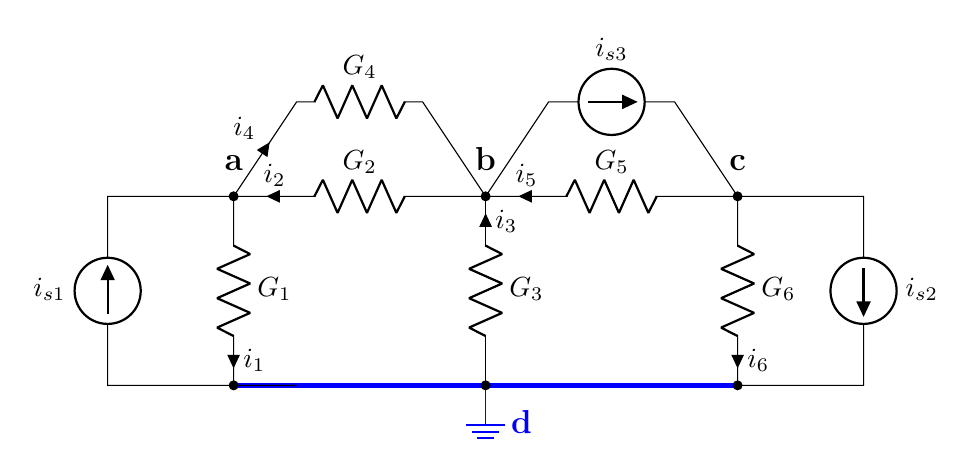
\begin{tikzpicture}[american, scale=0.8]
    % --- Définition des coordonnées ---
    \coordinate (d) at (0,0);
    \coordinate (a) at (-4,3);
    \coordinate (b) at (0,3);
    \coordinate (c) at (4,3);
    
    % --- Ligne de masse (Node d) ---
    \draw [blue, ultra thick] (a |- d) -- (c |- d);
    \node[blue, ground, scale=1.2] at (d) {};
    \node[blue, below right=2mm] at (d) {\large \textbf{d}};

    % --- Branche de gauche ---
    % Source is1
    \draw (-3, 0) -- (-6,0) to[I, l=$i_{s1}$] (-6,3) -- (a);
    % Résistance G1
    \draw (a) to[R, l=$G_1$, *-, i=$i_1$] (a |- d) node[circ]{};
    \node[above=2mm] at (a) {\large \textbf{a}};

    % --- Entre les nœuds a et b ---
    % Branche supérieure (G4)
    \draw (a) to[short, i=$i_4$] (-3,4.5) to[R, l=$G_4$] (-1,4.5) -- (b);
    % Branche centrale (G2)
    \draw (a) to[R, l=$G_2$, i<=$i_2$] (b);
    
    % --- Nœud b et branche centrale ---
    \node[above=2mm] at (b) {\large \textbf{b}};
    \draw (b) node[circ]{} to[R, l=$G_3$, i<=$i_3$] (d) node[circ]{};

    % --- Entre les nœuds b et c ---
    % Branche supérieure (is3)
    \draw (b) -- (1,4.5) to[I, l=$i_{s3}$] (3,4.5) -- (c);
    % Branche centrale (G5)
    \draw (b) to[R, l=$G_5$, i<=$i_5$] (c);

    % --- Branche de droite ---
    \node[above = 2mm] at (c) {\large \textbf{c}};
    % Résistance G6
    \draw (c) node[circ]{} to[R, l=$G_6$, i=$i_6$] (c |- d) node[circ]{};
    % Source is2
    \draw (c) -- (6,3) to[I, l=$i_{s2}$] (6,0) -- (c |- d);
\end{tikzpicture}

\end{document}